%% Creator: Inkscape 1.0.2 (e86c870879, 2021-01-15, custom), www.inkscape.org
%% PDF/EPS/PS + LaTeX output extension by Johan Engelen, 2010
%% Accompanies image file 'fig2.pdf' (pdf, eps, ps)
%%
%% To include the image in your LaTeX document, write
%%   \input{<filename>.pdf_tex}
%%  instead of
%%   \includegraphics{<filename>.pdf}
%% To scale the image, write
%%   \def\svgwidth{<desired width>}
%%   \input{<filename>.pdf_tex}
%%  instead of
%%   \includegraphics[width=<desired width>]{<filename>.pdf}
%%
%% Images with a different path to the parent latex file can
%% be accessed with the `import' package (which may need to be
%% installed) using
%%   \usepackage{import}
%% in the preamble, and then including the image with
%%   \import{<path to file>}{<filename>.pdf_tex}
%% Alternatively, one can specify
%%   \graphicspath{{<path to file>/}}
%% 
%% For more information, please see info/svg-inkscape on CTAN:
%%   http://tug.ctan.org/tex-archive/info/svg-inkscape
%%
\begingroup%
  \makeatletter%
  \providecommand\color[2][]{%
    \errmessage{(Inkscape) Color is used for the text in Inkscape, but the package 'color.sty' is not loaded}%
    \renewcommand\color[2][]{}%
  }%
  \providecommand\transparent[1]{%
    \errmessage{(Inkscape) Transparency is used (non-zero) for the text in Inkscape, but the package 'transparent.sty' is not loaded}%
    \renewcommand\transparent[1]{}%
  }%
  \providecommand\rotatebox[2]{#2}%
  \newcommand*\fsize{\dimexpr\f@size pt\relax}%
  \newcommand*\lineheight[1]{\fontsize{\fsize}{#1\fsize}\selectfont}%
  \ifx\svgwidth\undefined%
    \setlength{\unitlength}{195.27076845bp}%
    \ifx\svgscale\undefined%
      \relax%
    \else%
      \setlength{\unitlength}{\unitlength * \real{\svgscale}}%
    \fi%
  \else%
    \setlength{\unitlength}{\svgwidth}%
  \fi%
  \global\let\svgwidth\undefined%
  \global\let\svgscale\undefined%
  \makeatother%
  \begin{picture}(1,0.5215872)%
    \lineheight{1}%
    \setlength\tabcolsep{0pt}%
    \put(0,0){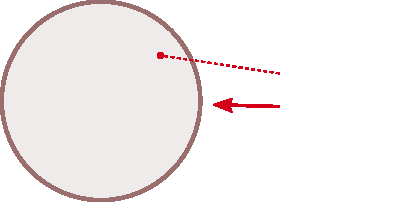
\includegraphics[width=\unitlength,page=1]{waveoptics/scheme/fig2.pdf}}%
    \put(0.92645221,0.21560272){\makebox(0,0)[lt]{\lineheight{1.25}\smash{\begin{tabular}[t]{l}$\bfR_k$\end{tabular}}}}%
    \put(0.56274836,0.21221995){\makebox(0,0)[lt]{\lineheight{1.25}\smash{\begin{tabular}[t]{l}$\hatbfR_{\Cls k}$\end{tabular}}}}%
    \put(0.33172694,0.34184498){\makebox(0,0)[lt]{\lineheight{1.25}\smash{\begin{tabular}[t]{l}$\bfR_i$\end{tabular}}}}%
    \put(0.15998663,0.24282036){\makebox(0,0)[lt]{\lineheight{1.25}\smash{\begin{tabular}[t]{l}$\bfR_\Cls$\end{tabular}}}}%
    \put(0,0){\includegraphics[width=\unitlength,page=2]{waveoptics/scheme/fig2.pdf}}%
    \put(0.47642379,0.08204267){\makebox(0,0)[lt]{\lineheight{1.25}\smash{\begin{tabular}[t]{l}$R_{\Cls k}$\end{tabular}}}}%
    \put(0,0){\includegraphics[width=\unitlength,page=3]{waveoptics/scheme/fig2.pdf}}%
    \put(0.59047783,0.30130627){\makebox(0,0)[lt]{\lineheight{1.25}\smash{\begin{tabular}[t]{l}$\hatbfR_{ik}$\end{tabular}}}}%
    \put(0.07747599,0.39359056){\makebox(0,0)[lt]{\lineheight{1.25}\smash{\begin{tabular}[t]{l}$\Cls$\end{tabular}}}}%
    \put(0,0){\includegraphics[width=\unitlength,page=4]{waveoptics/scheme/fig2.pdf}}%
  \end{picture}%
\endgroup%
